\documentclass[12pt,]{article}
\usepackage{lmodern}
\usepackage{amssymb,amsmath}
\usepackage{ifxetex,ifluatex}
\usepackage{fixltx2e} % provides \textsubscript
\ifnum 0\ifxetex 1\fi\ifluatex 1\fi=0 % if pdftex
  \usepackage[T1]{fontenc}
  \usepackage[utf8]{inputenc}
\else % if luatex or xelatex
  \ifxetex
    \usepackage{mathspec}
  \else
    \usepackage{fontspec}
  \fi
  \defaultfontfeatures{Ligatures=TeX,Scale=MatchLowercase}
    \setmainfont[]{Times New Roman}
    \setsansfont[]{Times New Roman}
\fi
% use upquote if available, for straight quotes in verbatim environments
\IfFileExists{upquote.sty}{\usepackage{upquote}}{}
% use microtype if available
\IfFileExists{microtype.sty}{%
\usepackage{microtype}
\UseMicrotypeSet[protrusion]{basicmath} % disable protrusion for tt fonts
}{}
\usepackage[margin=2.5cm]{geometry}
\usepackage{hyperref}
\hypersetup{unicode=true,
            pdftitle={Regressão espacial com o uso do R},
            pdfauthor={Luiz Fernando Palin Droubi; Willian Zonato},
            pdfborder={0 0 0},
            breaklinks=true}
\urlstyle{same}  % don't use monospace font for urls
\usepackage{color}
\usepackage{fancyvrb}
\newcommand{\VerbBar}{|}
\newcommand{\VERB}{\Verb[commandchars=\\\{\}]}
\DefineVerbatimEnvironment{Highlighting}{Verbatim}{commandchars=\\\{\}}
% Add ',fontsize=\small' for more characters per line
\usepackage{framed}
\definecolor{shadecolor}{RGB}{248,248,248}
\newenvironment{Shaded}{\begin{snugshade}}{\end{snugshade}}
\newcommand{\KeywordTok}[1]{\textcolor[rgb]{0.13,0.29,0.53}{\textbf{#1}}}
\newcommand{\DataTypeTok}[1]{\textcolor[rgb]{0.13,0.29,0.53}{#1}}
\newcommand{\DecValTok}[1]{\textcolor[rgb]{0.00,0.00,0.81}{#1}}
\newcommand{\BaseNTok}[1]{\textcolor[rgb]{0.00,0.00,0.81}{#1}}
\newcommand{\FloatTok}[1]{\textcolor[rgb]{0.00,0.00,0.81}{#1}}
\newcommand{\ConstantTok}[1]{\textcolor[rgb]{0.00,0.00,0.00}{#1}}
\newcommand{\CharTok}[1]{\textcolor[rgb]{0.31,0.60,0.02}{#1}}
\newcommand{\SpecialCharTok}[1]{\textcolor[rgb]{0.00,0.00,0.00}{#1}}
\newcommand{\StringTok}[1]{\textcolor[rgb]{0.31,0.60,0.02}{#1}}
\newcommand{\VerbatimStringTok}[1]{\textcolor[rgb]{0.31,0.60,0.02}{#1}}
\newcommand{\SpecialStringTok}[1]{\textcolor[rgb]{0.31,0.60,0.02}{#1}}
\newcommand{\ImportTok}[1]{#1}
\newcommand{\CommentTok}[1]{\textcolor[rgb]{0.56,0.35,0.01}{\textit{#1}}}
\newcommand{\DocumentationTok}[1]{\textcolor[rgb]{0.56,0.35,0.01}{\textbf{\textit{#1}}}}
\newcommand{\AnnotationTok}[1]{\textcolor[rgb]{0.56,0.35,0.01}{\textbf{\textit{#1}}}}
\newcommand{\CommentVarTok}[1]{\textcolor[rgb]{0.56,0.35,0.01}{\textbf{\textit{#1}}}}
\newcommand{\OtherTok}[1]{\textcolor[rgb]{0.56,0.35,0.01}{#1}}
\newcommand{\FunctionTok}[1]{\textcolor[rgb]{0.00,0.00,0.00}{#1}}
\newcommand{\VariableTok}[1]{\textcolor[rgb]{0.00,0.00,0.00}{#1}}
\newcommand{\ControlFlowTok}[1]{\textcolor[rgb]{0.13,0.29,0.53}{\textbf{#1}}}
\newcommand{\OperatorTok}[1]{\textcolor[rgb]{0.81,0.36,0.00}{\textbf{#1}}}
\newcommand{\BuiltInTok}[1]{#1}
\newcommand{\ExtensionTok}[1]{#1}
\newcommand{\PreprocessorTok}[1]{\textcolor[rgb]{0.56,0.35,0.01}{\textit{#1}}}
\newcommand{\AttributeTok}[1]{\textcolor[rgb]{0.77,0.63,0.00}{#1}}
\newcommand{\RegionMarkerTok}[1]{#1}
\newcommand{\InformationTok}[1]{\textcolor[rgb]{0.56,0.35,0.01}{\textbf{\textit{#1}}}}
\newcommand{\WarningTok}[1]{\textcolor[rgb]{0.56,0.35,0.01}{\textbf{\textit{#1}}}}
\newcommand{\AlertTok}[1]{\textcolor[rgb]{0.94,0.16,0.16}{#1}}
\newcommand{\ErrorTok}[1]{\textcolor[rgb]{0.64,0.00,0.00}{\textbf{#1}}}
\newcommand{\NormalTok}[1]{#1}
\usepackage{graphicx,grffile}
\makeatletter
\def\maxwidth{\ifdim\Gin@nat@width>\linewidth\linewidth\else\Gin@nat@width\fi}
\def\maxheight{\ifdim\Gin@nat@height>\textheight\textheight\else\Gin@nat@height\fi}
\makeatother
% Scale images if necessary, so that they will not overflow the page
% margins by default, and it is still possible to overwrite the defaults
% using explicit options in \includegraphics[width, height, ...]{}
\setkeys{Gin}{width=\maxwidth,height=\maxheight,keepaspectratio}
\IfFileExists{parskip.sty}{%
\usepackage{parskip}
}{% else
\setlength{\parindent}{0pt}
\setlength{\parskip}{6pt plus 2pt minus 1pt}
}
\setlength{\emergencystretch}{3em}  % prevent overfull lines
\providecommand{\tightlist}{%
  \setlength{\itemsep}{0pt}\setlength{\parskip}{0pt}}
\setcounter{secnumdepth}{5}
% Redefines (sub)paragraphs to behave more like sections
\ifx\paragraph\undefined\else
\let\oldparagraph\paragraph
\renewcommand{\paragraph}[1]{\oldparagraph{#1}\mbox{}}
\fi
\ifx\subparagraph\undefined\else
\let\oldsubparagraph\subparagraph
\renewcommand{\subparagraph}[1]{\oldsubparagraph{#1}\mbox{}}
\fi

%%% Use protect on footnotes to avoid problems with footnotes in titles
\let\rmarkdownfootnote\footnote%
\def\footnote{\protect\rmarkdownfootnote}

%%% Change title format to be more compact
\usepackage{titling}

% Create subtitle command for use in maketitle
\newcommand{\subtitle}[1]{
  \posttitle{
    \begin{center}\large#1\end{center}
    }
}

\setlength{\droptitle}{-2em}
  \title{Regressão espacial com o uso do R}
  \pretitle{\vspace{\droptitle}\centering\huge}
  \posttitle{\par}
  \author{Luiz Fernando Palin Droubi \\ Willian Zonato}
  \preauthor{\centering\large\emph}
  \postauthor{\par}
  \predate{\centering\large\emph}
  \postdate{\par}
  \date{21 de fevereiro de 2018}

\usepackage{sectsty} \sectionfont{\fontsize{12}{15}\selectfont}
\usepackage[brazil]{babel}
\usepackage{graphicx}
\usepackage{float}
\usepackage{subfig}
\usepackage{caption}

\begin{document}
\maketitle

\subsection*{Resumo}\label{resumo}
\addcontentsline{toc}{subsection}{Resumo}

\emph{Os modelos estatísticos espaciais, notadamente os modelos de
regressão espacial e geoestatísticos, vem sendo progressivamente cada
vez mais utilizados nas avaliações de imóveis. O uso de modelos de
regressão linear com dados espaciais são sempre suspeitos: a
possibilidade de autocorrelação espacial dos resíduos é grande, ainda
mais na área de avaliação de imóveis urbanos, onde a variável
localização é sabidamente importante na imensa maioria dos centros
urbanos. Atualmente, como meio de contornar este problema, a maioria dos
avaliadores adota a criação de variáveis de distância a polos de
valorização, mas isto requer um conhecimento detalhado do local por
parte do avaliador e nem sempre estas variáveis podem ser definidas
precisamente, ou ainda, enquanto captam a influência da proximidade de
um determinado polo, deixam escapar a influência de outros fatores de
valorização. No entanto, na regressão espacial, há a dificuldade
computacional (necessidade de softwares específicos, treinamento, etc.).
Pretende-se demonstrar neste artigo como os avaliadores podem fazer uso
da poderosa linguagem \textbf{R} para a utilização da regressão
espacial, com uma curva de aprendizado suave.}

\textbf{\emph{Palavras-chave}}: \emph{Regressão Espacial. Avaliação de
imóveis. Inferência}

\section{INTRODUÇÃO}\label{introducao}

Segundo TRIVELLONI (\protect\hyperlink{ref-trivelloni07}{2007}),

\begin{quote}
os modelos tradicionais de inferência estatística mostram dificuldades
para lidar de maneira eficiente com os efeitos espaciais nos dados; as
variáveis de localização, quando não são corretamente especificadas nos
modelos, além da perda de poder explicativo dos modelos produzem
autocorrelação espacial nos resíduos da regressão, invalidando seus
resultados.
\end{quote}

A grande maioria dos avaliadores na atualidade utiliza os modelos
tradicionais de inferência estatística, que:

\begin{quote}
mostram dificuldades para lidar de maneira eficiente com os efeitos
espaciais nos dados; as variáveis de localização, quando não são
corretamente especificadas nos modelos, além da perda de poder
explicativo dos modelos produzem autocorrelação espacial nos resíduos da
regressão, invalidando seus resultados(TRIVELLONI
\protect\hyperlink{ref-trivelloni07}{2007}).
\end{quote}

Porém, é sabido que ``os modelos de inferência tradicional podem também
alcançar resultados adequados se as variáveis explicativas que tem
estrutura espacial forem corretamente especificadas no
modelo.''(TRIVELLONI \protect\hyperlink{ref-trivelloni07}{2007})

Desta maneira, é possível que sejam combinadas as técnicas da inferência
estatística tradicional com técnicas espaciais para a especificação da
compenente espacial do valor, produzindo assim um ``modelo híbrido.''

Ainda de acordo com TRIVELLONI
(\protect\hyperlink{ref-trivelloni07}{2007}), ``vários trabalhos têm
mostrado que esta combinação pode produzir melhores resultados que os
conseguidos com cada método de forma isolada.''

\section{REVISÃO BIBLIOGRÁFICA}\label{revisao-bibliografica}

\subsection{Inferência estatística}\label{inferencia-estatistica}

Segundo SARMIENTO-BARBIERI
(\protect\hyperlink{ref-sarmiento-barbieri}{2016}), ``o método
tradicional, por muitos anos, tem sido ignorar a dependência espacial
dos dados e apenas rodar uma regressão linear'' do tipo:

\begin{equation}
  \label{eq-OLS}
  Y = X\beta + \epsilon
\end{equation}

\begin{quote}
O problema em ignorar a estrutura espacial dos dados implica que as
estimativas da regressão linear no modelo não-espacial podem estar
enviesadas, inconsistentes ou ineficientes, dependendo de qual é a real
dependência (dos dados espaciais)(SARMIENTO-BARBIERI
\protect\hyperlink{ref-sarmiento-barbieri}{2016}).
\end{quote}

\subsection{Modelando a dependência
espacial}\label{modelando-a-dependencia-espacial}

Autocorrelação espacial mede o quanto um dado fenômeno de interesse está
correlacionado consigo mesmo no Espaço (Cliff and Ord (1973) apud
SARMIENTO-BARBIERI (\protect\hyperlink{ref-sarmiento-barbieri}{2016})).

SARMIENTO-BARBIERI (\protect\hyperlink{ref-sarmiento-barbieri}{2016})
salienta que a autocorrelação espacial pode ser positiva, ou seja,
valores similares aparecem sempre próximos uns dos outros, formando um
\emph{cluster}, ou negativa, ou seja, dados vizinhos são dissimilares.

Segundo ANSELIN (apud SARMIENTO-BARBIERI
(\protect\hyperlink{ref-sarmiento-barbieri}{2016})), pode-se expressar a
existência de autocorrelação espacial com a seguinte condição de
momentos:

\begin{equation}
  \label{eq-cov}
  Cov(y_i,y_j) \neq  0\ para\ i \neq  j
\end{equation}

onde \(y_i\) and \(y_j\) são observações de uma variável aleatória nos
locais \(i\) e \(j\).

Para SARMIENTO-BARBIERI
(\protect\hyperlink{ref-sarmiento-barbieri}{2016}), ``o problema então
seria estimar a matriz de covariância \(N\) x \(N\) diretamente para
\(N\) observações.''

\begin{quote}
Para contornar esse problema, impomos restrições à natureza das
interações. Um tipo de restrição é definir para cada ponto de dados um
``conjunto de vizinhança'' relevante. Na econometria espacial, isto é
operacionalizado através da \textbf{matriz espacial de pesos}.
\end{quote}

Esta nada mais é do que uma matriz simétrica em que para cada observação
(linhas) indica os locais de vizinhança (colunas) através de elementos
não-nulos. Ou seja, os elementos \(w_{ij}\) da matriz espacial de pesos
\(W\) serão computados da seguinte forma:

\begin{equation}
  \label{eq-W}
  [w_{ij}] = \left\{\begin{matrix}
  1 & se & j \in N(i)\\ 
  0 & 
\end{matrix}\right.
\end{equation}

onde \(N(i)\) é o conjunto de dados vizinhos da observação \(i\).

Outro procedimento viável é definir dois dados como vizinhos se eles
obedecem um mesmo critério de distância, isto é, \(j \in N(j)\) se
\(d_{ij} < d_{max}\), onde \(d\) é a distância entre os dados \(i\) e
\(j\).

\subsection{Modelos de regressão
espacial}\label{modelos-de-regressao-espacial}

Segundo TRIVELLONI (\protect\hyperlink{ref-trivelloni07}{2007}), os
principais modelos de regressão utilizados na econometria espacial são o
Modelo da Variável Dependente e o Modelo Espacial do Erro.

Nesta seção veremos as principais características de cada modelo e sua
formulação.

\subsubsection{Modelos espaciais autoregressivos ou Modelo da Variável
Dependente}\label{modelos-espaciais-autoregressivos-ou-modelo-da-variavel-dependente}

A dependência espacial pode ser modelada em uma regressão linear de
forma semelhante a um processo autorregressivo em séries temporais.
Segundo SARMIENTO-BARBIERI
(\protect\hyperlink{ref-sarmiento-barbieri}{2016}), isto pode ser
escrito formalmente como na equação abaixo:

\begin{equation}
  \label{eq-SAR}
  y = \rho Wy + X \beta + \epsilon
\end{equation}

Vê-se na equação \ref{eq-SAR}, que além dos termos da equação
\ref{eq-OLS}, tem-se um termo adicional (\(\rho Wy\)), que é justamente
o termo que modela a autocorrelação da variável dependente (\(y\)), em
que \(W\) é a matriz de pesos espaciais e\(\rho\) é o parâmetro (a ser
estimado) de autocorrelação espacial da variável dependente.

Porém, de acordo com ANSELIN (apud SARMIENTO-BARBIERI
(\protect\hyperlink{ref-sarmiento-barbieri}{2016})), ao contrário das
séries temporais, nas correlações espaciais os \([Wy]_i\) estão sempre
correlacionados com os \(\epsilon_i\) independentemente da estrutura dos
erros. Isto implica que as estimativas no modelo não-espacial estarão
enviesadas e inconsistentes.

\subsubsection{Modelo espacial do erro}\label{modelo-espacial-do-erro}

Os modelos deste tipo se apresentam na forma de uma regressão linear
ordinária (RLO), porém aqui a variável dos erros \(\epsilon\) é
espacialmente autocorrelacionada, como podemos notar na equação
\ref{eq-SEM-error}, ao contrário da RLO, onde a variável \(\epsilon\) é
aleatória, com distribuição normal e média zero.

\begin{equation}
  \label{eq-SEM}
  y = X\beta + \epsilon
\end{equation}

Com:

\begin{equation}
  \label{eq-SEM-error}
  \epsilon = \lambda W \epsilon + u
\end{equation}

\subsection{Modelos geoestatísticos}\label{modelos-geoestatisticos}

Segundo TRIVELLONI (\protect\hyperlink{ref-trivelloni07}{2007}), ``os
modelos geostatísticos buscam representar e modelar a variação espacial
de uma variável regionalizada''.

Variável regionalizada, ou seja, uma variável aleatória (\(Z\)) em que
há dependência entre seu valor e sua localização espacial, pode ser
expressa como(TRIVELLONI \protect\hyperlink{ref-trivelloni07}{2007}):

\begin{equation}
  \label{eq-regional}
  Z(x) = \mu(x) + \epsilon'(x) + \epsilon''
\end{equation}

onde x representa uma posição em uma, duas ou três dimensões; \(\mu(x)\)
é uma função determinística que descreve a componente estrutural de
\(Z\) em \(x\); \(\epsilon'(x)\) é um termo estocástico correlacionado
que varia localmente e \(\epsilon''\) é um ruído aleatório não
correlacionado, com distribuição normal, média zero e variância
\(\sigma^2\).

Desta forma, pode-se definir o estimador de krigagem (\(Z_k\)), como a
combinação linear dos \(Z(x_i)\) e os ponderadores \(\lambda_i\), da
seguinte maneira(TRIVELLONI \protect\hyperlink{ref-trivelloni07}{2007}):

\begin{equation}
  \label{eq-krigagem}
  Z_k = \sum{\lambda_i Z_i}
\end{equation}

onde os ponderadores \(\lambda_i\) são obtidos de forma que o estimador
\(Z_k\) seja ótimo, ou seja, a variância do erro seja mínima

\subsection{Testes de detecção de autocorrelação
espacial}\label{testes-de-deteccao-de-autocorrelacao-espacial}

\subsubsection{Teste I de Moran}\label{teste-i-de-moran}

Análogo ao teste de Durbin-Watson, porém em versão bidimensional:

\begin{equation}
  \label{eq-moran}
  I = \frac{e'We}{e'e}
\end{equation}

onde \(e = y - \beta X\), \(\beta = ({X}'X)^{-1}X'y\) e \(W\) é a matriz
de pesos espaciais.

A estatística em pauta depende da escolha da matriz \(W\).

\subsubsection{Teste do multiplicador de
Lagrange}\label{teste-do-multiplicador-de-lagrange}

Embora o teste de Moran tenha a interessante característica de ter um
alto poder contra uma ampla gama de alternativas (ANSELIN apud
SARMIENTO-BARBIERI (\protect\hyperlink{ref-sarmiento-barbieri}{2016}), o
teste não dá parâmetros para a escolha de modelos alternativos.

Por outro lado, o teste do multiplicador de Lagrange especifica as
hipóteses alternativas de autocorrelação espacial da variável dependente
e da autocorrelação espacial dos resíduos, o que pode ser útil nestes
casos.

\section{DESENVOLVIMENTO}\label{desenvolvimento}

Nesta seção são desenvolvidos dois exemplos do uso das ténicas de
regressão espacial usando o R, com o intuito de demonstrar como este
\emph{software} pode ser utilizado para facilmente aplicar as teorias da
econometria espacial.

O primeiro exemplo foi extraído de SARMIENTO-BARBIERI
(\protect\hyperlink{ref-sarmiento-barbieri}{2016}), dados de crimes
violentos são correlacionados com dados de execução de hipotecas e de
desemprego na cidade de Chicago (EUA).

E o segundo exemplo, aplicado à área de avaliação de imóveis, onde dados
censitários de 2000 na Califórnia (EUA) são utilizados para estudo da
autocorrelação espacial dos valores dos imóveis.

\subsection{Exemplo 1}\label{exemplo-1}

O exemplo abaixo é reproduzido de SARMIENTO-BARBIERI
(\protect\hyperlink{ref-sarmiento-barbieri}{2016}). Os dados aqui
utilizados aqui podem ser obtidos no sítio
\href{http://www.econ.uiuc.edu/~lab/workshop/foreclosures/}{www.econ.uiuc.edu/\textasciitilde{}lab/workshop/foreclosures/}.

De posse dos arquivos, primeiramente, deve-se fazer a leitura do
\emph{shapefile} dentro do sistema \emph{R}, através da função
\texttt{readOGR} do pacote \texttt{rgdal}.

\begin{Shaded}
\begin{Highlighting}[]
\NormalTok{chi.poly <-}\StringTok{ }\KeywordTok{readOGR}\NormalTok{(}\StringTok{'./shapefiles/foreclosures.shp'}\NormalTok{)}
\end{Highlighting}
\end{Shaded}

\begin{verbatim}
## OGR data source with driver: ESRI Shapefile 
## Source: "./shapefiles/foreclosures.shp", layer: "foreclosures"
## with 897 features
## It has 16 fields
\end{verbatim}

O \emph{shapefile} é um arquivo repleto de dados, não apenas espaciais,
mas também dados de variáveis de interesse, todas elas
georreferenciadas. Por exemplo, abaixo pode ser visto um pequeno resumo
dos dados encontrados no \emph{shapefile} carregado:

\begin{Shaded}
\begin{Highlighting}[]
\KeywordTok{str}\NormalTok{(chi.poly, }\DataTypeTok{max.level =} \DecValTok{2}\NormalTok{)}
\end{Highlighting}
\end{Shaded}

\begin{verbatim}
## Formal class 'SpatialPolygonsDataFrame' [package "sp"] with 5 slots
##   ..@ data       :'data.frame':  897 obs. of  16 variables:
##   ..@ polygons   :List of 897
##   ..@ plotOrder  : int [1:897] 643 865 885 657 864 866 658 659 873 889 ...
##   ..@ bbox       : num [1:2, 1:2] -87.9 41.6 -87.5 42
##   .. ..- attr(*, "dimnames")=List of 2
##   ..@ proj4string:Formal class 'CRS' [package "sp"] with 1 slot
\end{verbatim}

Percebemos no resumo acima que, no objeto \emph{chi.poly} estão contidos
um conjunto de dados (\emph{data.frame}) com 897 observações, um
conjunto de polígonos (\emph{polygons}) e um vetor com a sequência dos
pontos de cada polígono (\emph{plotOrder}).

Abaixo pode ser visto o gráfico produzido com os polígonos do
\emph{shapefile}.

\begin{Shaded}
\begin{Highlighting}[]
\KeywordTok{plot}\NormalTok{(chi.poly)}
\end{Highlighting}
\end{Shaded}

\begin{figure}[H]

{\centering 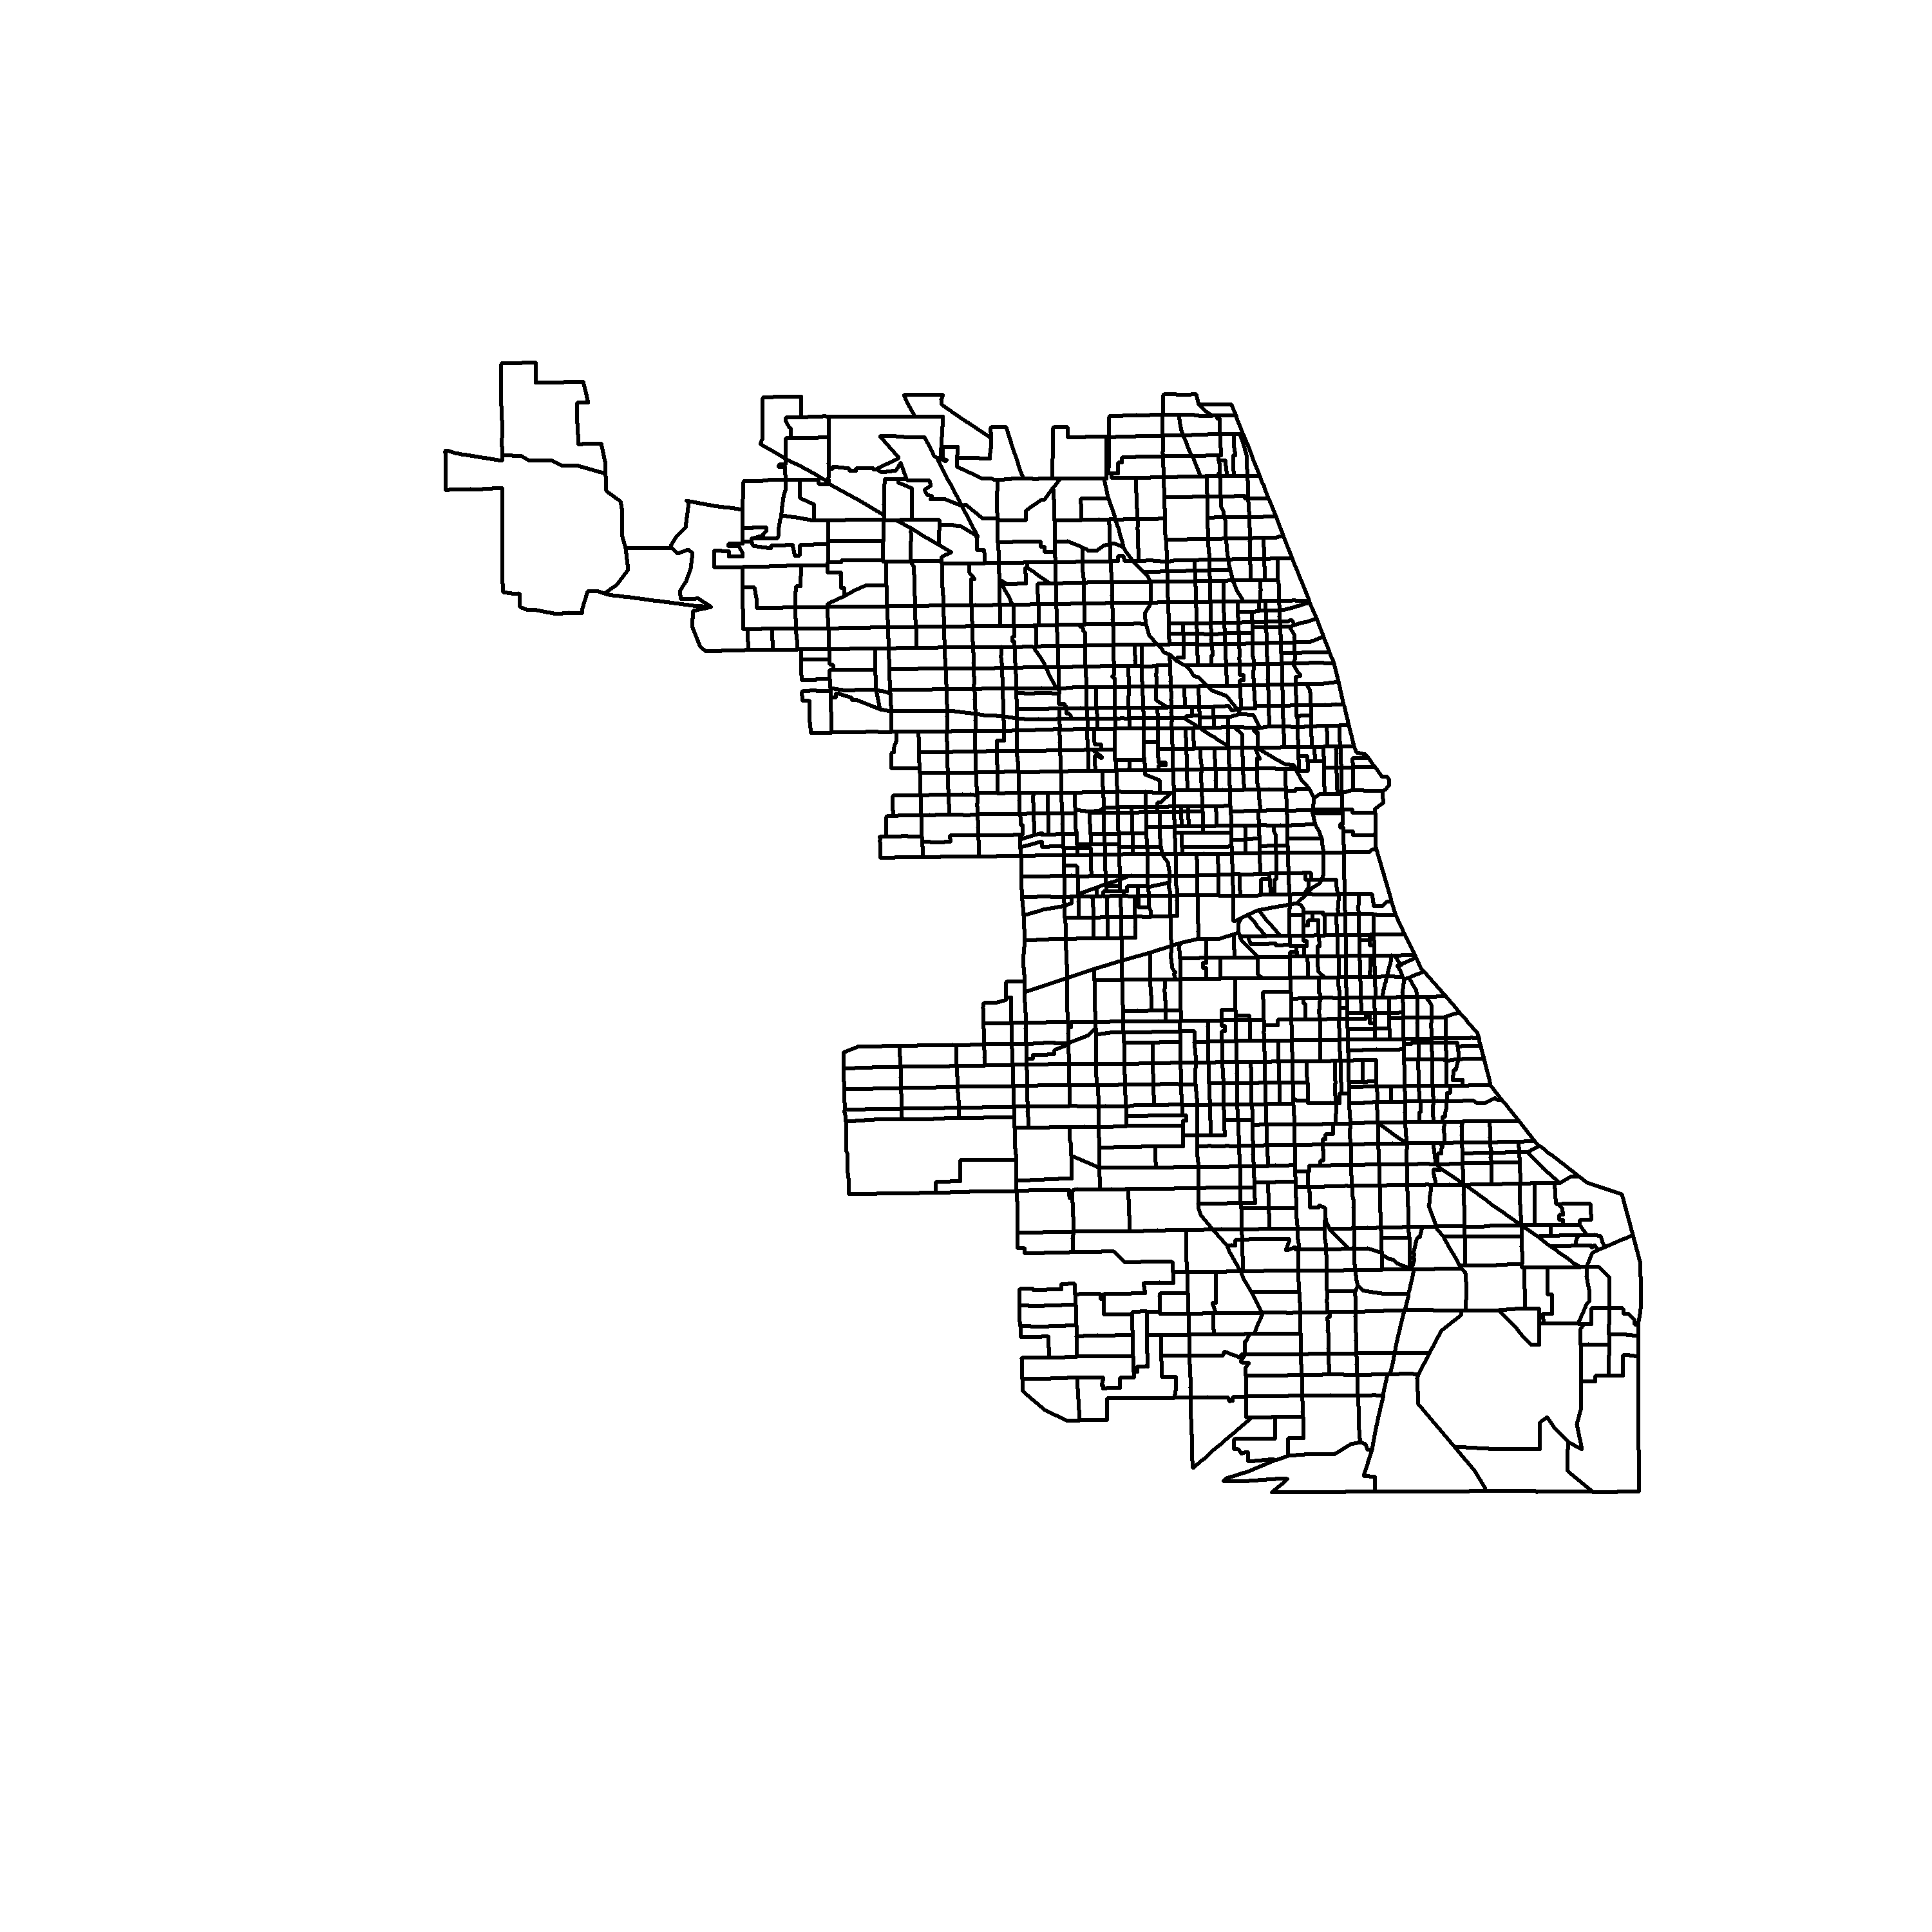
\includegraphics[width=0.65\linewidth]{sfiles/plot-1} 

}

\caption{Polígonos do \textit{shapefile}}\label{fig:plot}
\end{figure}

Estes polígonos encontram-se georreferenciados e todas as coordenadas
estão inclusas dentro de um \emph{boundary box} que pode ser encontrado
em:

\begin{Shaded}
\begin{Highlighting}[]
\NormalTok{chi.poly}\OperatorTok{@}\NormalTok{bbox}
\end{Highlighting}
\end{Shaded}

\begin{verbatim}
##         min       max
## x -87.94027 -87.52404
## y  41.64423  42.03793
\end{verbatim}

No \emph{R}, com o auxílio do pacote \texttt{ggmap}, pode-se criar uma
figura com os polígonos e um \emph{background} extraído do
\href{https://www.google.com.br/maps}{Google Maps}, preenchendo os
polígonos do \emph{shapefile} com a variável \emph{violent}, que contem
os dados de crimes violentos, para checar sua distribuição espacial:

\begin{Shaded}
\begin{Highlighting}[]
\NormalTok{chicago_map <-}\StringTok{ }\KeywordTok{get_map}\NormalTok{(}\DataTypeTok{location =}\NormalTok{ chi.poly}\OperatorTok{@}\NormalTok{bbox, }\DataTypeTok{maptype =} \StringTok{"terrain"}\NormalTok{,}
                       \DataTypeTok{source =} \StringTok{"google"}\NormalTok{)}
\NormalTok{chicago_poly <-}\StringTok{ }\KeywordTok{fortify}\NormalTok{(chi.poly, }\DataTypeTok{region =} \StringTok{'SP_ID'}\NormalTok{)}
\NormalTok{chicago_poly <-}\StringTok{ }\KeywordTok{merge}\NormalTok{(chicago_poly, chi.poly}\OperatorTok{@}\NormalTok{data, }\DataTypeTok{by.x =} \StringTok{'id'}\NormalTok{,}
                      \DataTypeTok{by.y =} \StringTok{'SP_ID'}\NormalTok{, }\DataTypeTok{all.x =} \OtherTok{TRUE}\NormalTok{)}
\NormalTok{p <-}\StringTok{ }\KeywordTok{ggmap}\NormalTok{(chicago_map) }\OperatorTok{+}\StringTok{ }\KeywordTok{geom_polygon}\NormalTok{(}\DataTypeTok{data =}\NormalTok{ chicago_poly,}
                                       \KeywordTok{aes}\NormalTok{(}\DataTypeTok{x =}\NormalTok{ long, }\DataTypeTok{y =}\NormalTok{ lat, }
                                           \DataTypeTok{group =}\NormalTok{ group, }\DataTypeTok{fill =}\NormalTok{ violent),}
                                       \DataTypeTok{size =}\NormalTok{ .}\DecValTok{2}\NormalTok{, }\DataTypeTok{color =} \StringTok{'green'}\NormalTok{) }\OperatorTok{+}\StringTok{ }
\StringTok{      }\KeywordTok{scale_fill_distiller}\NormalTok{(}\DataTypeTok{palette =} \StringTok{'Spectral'}\NormalTok{)}
\NormalTok{p}
\end{Highlighting}
\end{Shaded}

\begin{figure}[H]

{\centering 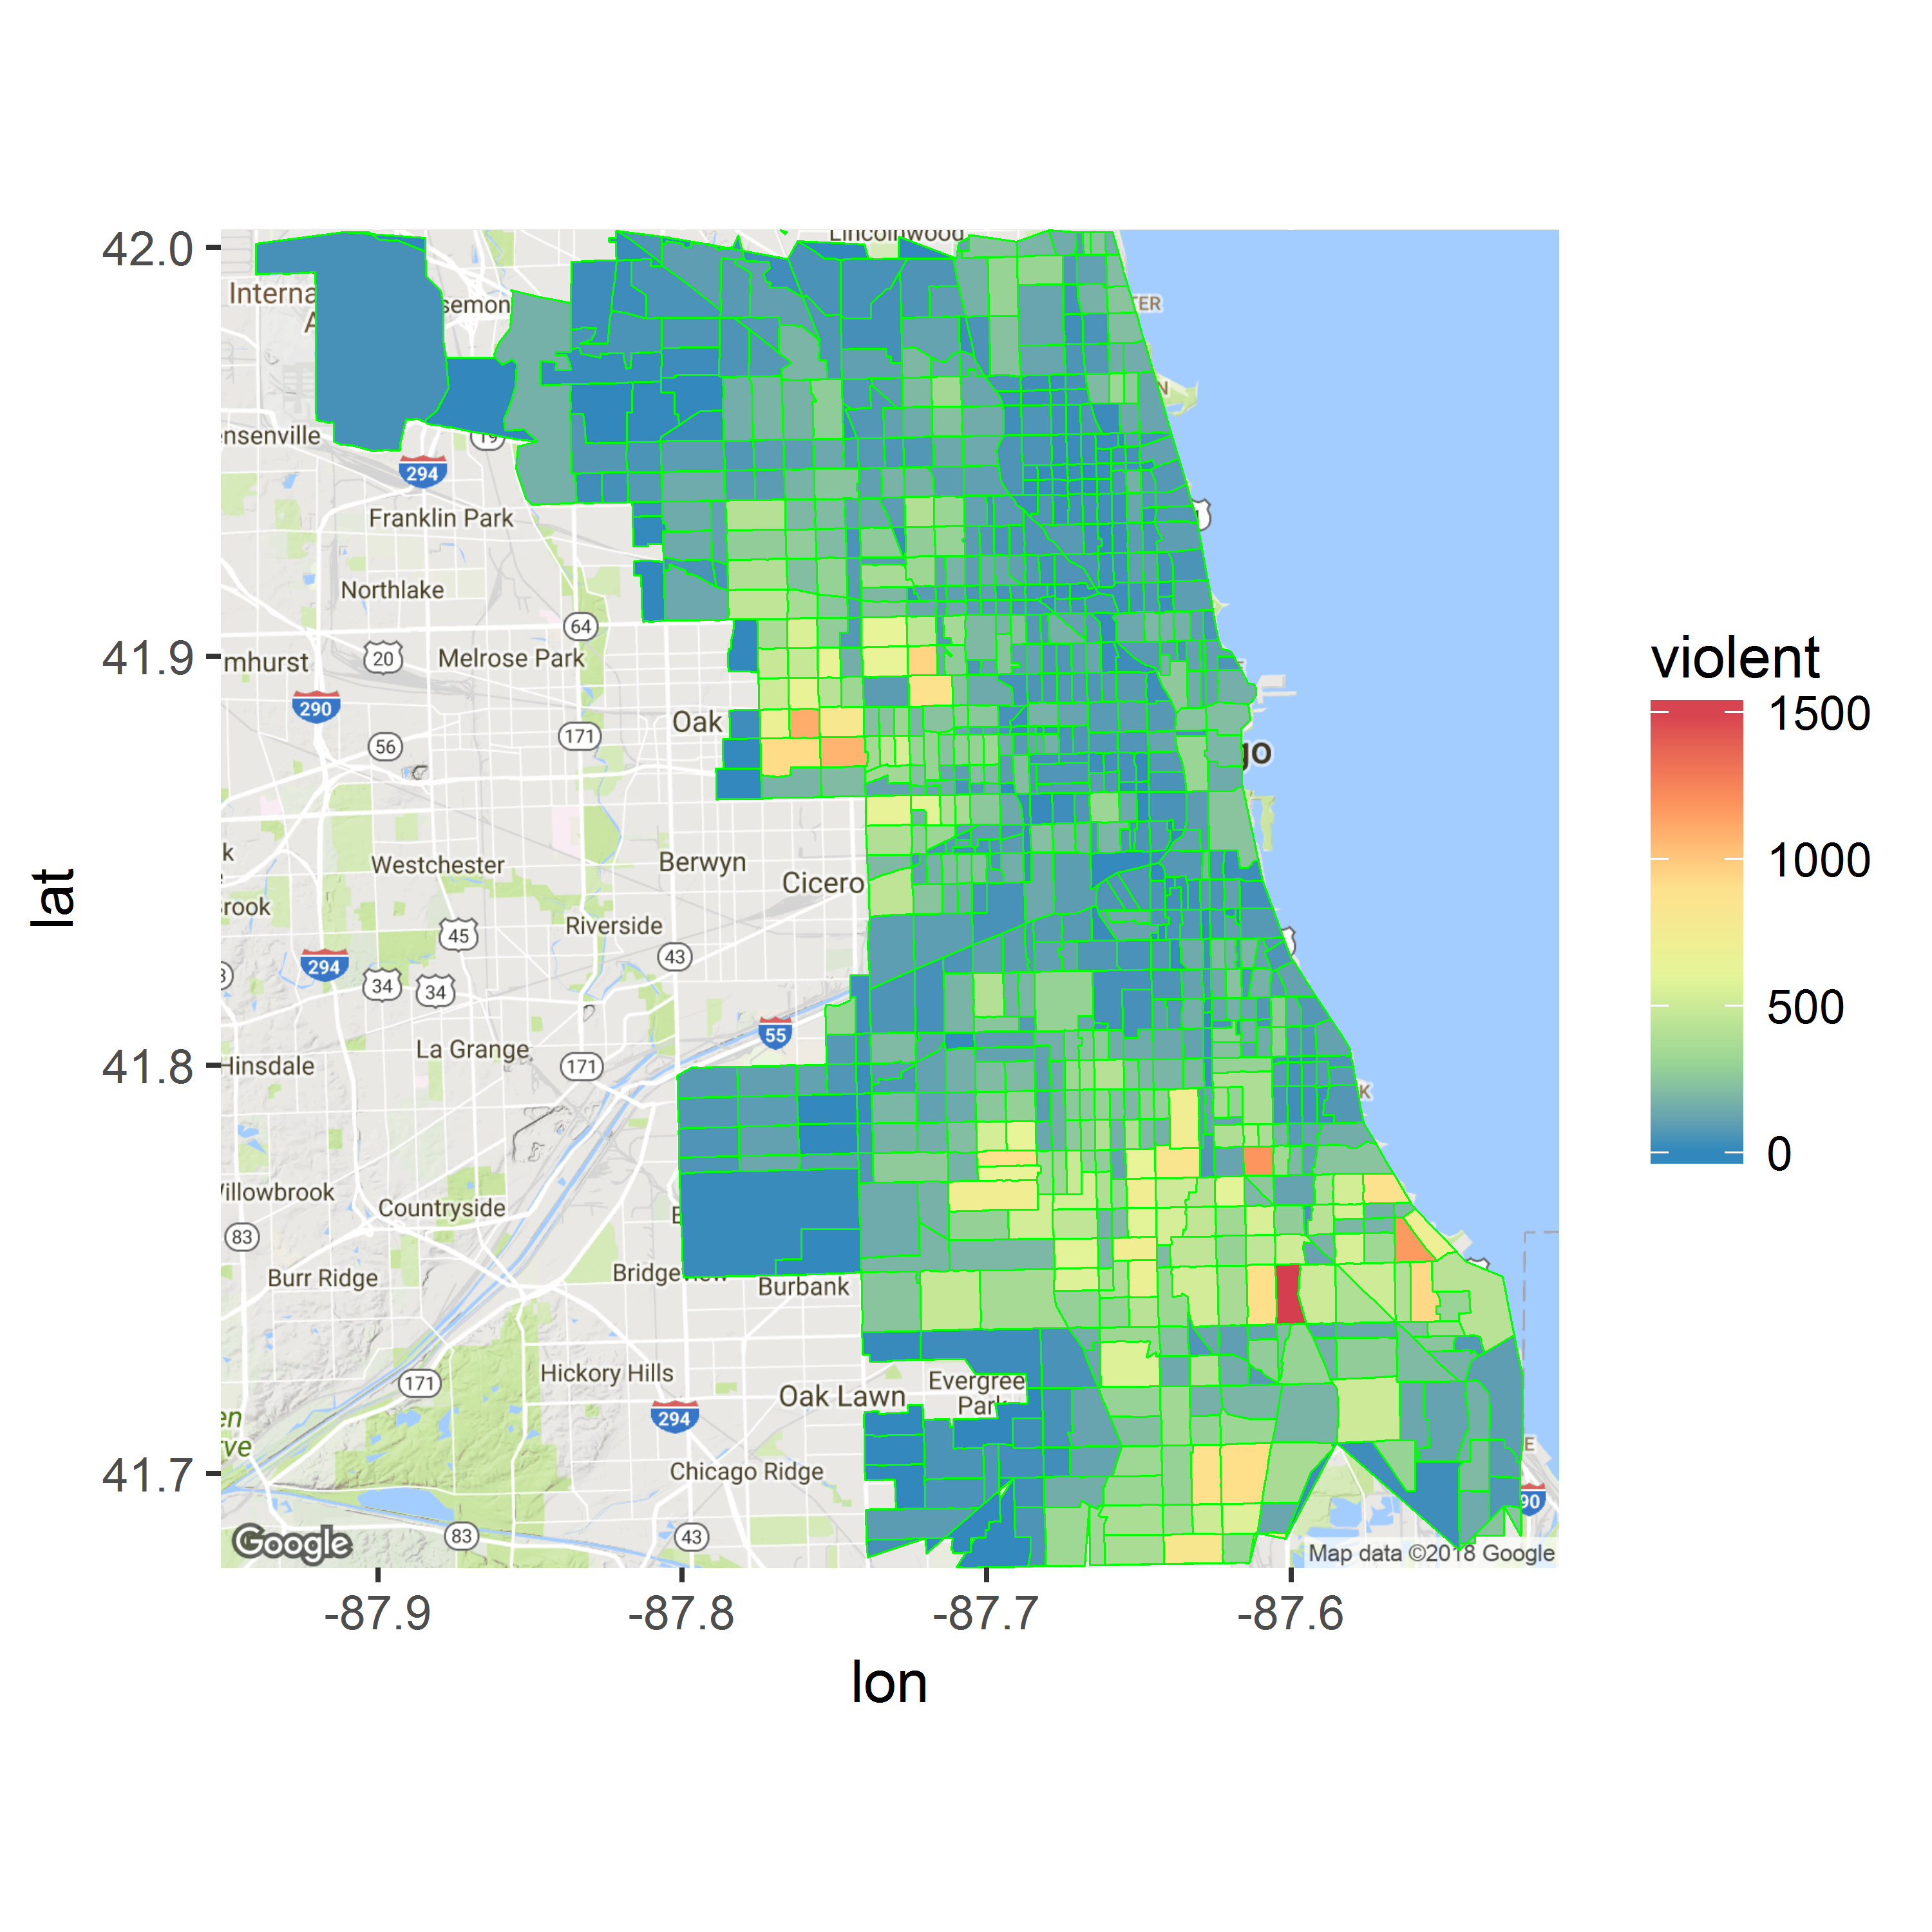
\includegraphics[width=0.65\linewidth]{sfiles/plot_mash-1} 

}

\caption{Distribuição dos crimes violentos na cidade de Chicago}\label{fig:plot_mash}
\end{figure}

No \emph{R}, a criação da matriz \(W\) é feita através do uso de duas
funções, como abaixo:

\begin{Shaded}
\begin{Highlighting}[]
\NormalTok{list.queen <-}\StringTok{ }\KeywordTok{poly2nb}\NormalTok{(chi.poly, }\DataTypeTok{queen =} \OtherTok{TRUE}\NormalTok{)}
\NormalTok{W <-}\StringTok{ }\KeywordTok{nb2listw}\NormalTok{(list.queen, }\DataTypeTok{style =} \StringTok{"W"}\NormalTok{, }\DataTypeTok{zero.policy =} \OtherTok{TRUE}\NormalTok{)}
\end{Highlighting}
\end{Shaded}

\subsection{Regressão Linear
Ordinária}\label{regressao-linear-ordinaria}

Apenas para ilustar, abaixo será apresentada uma regressão linear
ordinária dos dados do modelo, modelando a variável dependente
\emph{violent} contra as variáveis explicativas \emph{est\_fcs\_rt}, que
contem os dados de execução de hipotecas e a variável \emph{bls\_unemp},
que contem os dados sobre desemprego:

\begin{Shaded}
\begin{Highlighting}[]
\NormalTok{chi.ols <-}\StringTok{ }\KeywordTok{lm}\NormalTok{(violent }\OperatorTok{~}\StringTok{ }\NormalTok{est_fcs_rt }\OperatorTok{+}\StringTok{ }\NormalTok{bls_unemp, }\DataTypeTok{data =}\NormalTok{ chi.poly}\OperatorTok{@}\NormalTok{data)}
\KeywordTok{summary}\NormalTok{(chi.ols)}
\end{Highlighting}
\end{Shaded}

\begin{verbatim}
## 
## Call:
## lm(formula = violent ~ est_fcs_rt + bls_unemp, data = chi.poly@data)
## 
## Residuals:
##     Min      1Q  Median      3Q     Max 
## -892.02  -77.02  -23.73   41.90 1238.22 
## 
## Coefficients:
##             Estimate Std. Error t value Pr(>|t|)    
## (Intercept)  -18.627     45.366  -0.411    0.681    
## est_fcs_rt    28.298      1.435  19.720   <2e-16 ***
## bls_unemp     -0.308      5.770  -0.053    0.957    
## ---
## Signif. codes:  0 '***' 0.001 '**' 0.01 '*' 0.05 '.' 0.1 ' ' 1
## 
## Residual standard error: 157.3 on 894 degrees of freedom
## Multiple R-squared:  0.3141, Adjusted R-squared:  0.3126 
## F-statistic: 204.7 on 2 and 894 DF,  p-value: < 2.2e-16
\end{verbatim}

\subsection{Teste de Moran}\label{teste-de-moran}

\begin{Shaded}
\begin{Highlighting}[]
\NormalTok{moran.lm <-}\StringTok{ }\KeywordTok{lm.morantest}\NormalTok{(chi.ols, W, }\DataTypeTok{alternative =} \StringTok{"two.sided"}\NormalTok{)}
\NormalTok{moran.lm}
\end{Highlighting}
\end{Shaded}

\begin{verbatim}
## 
##  Global Moran I for regression residuals
## 
## data:  
## model: lm(formula = violent ~ est_fcs_rt + bls_unemp, data =
## chi.poly@data)
## weights: W
## 
## Moran I statistic standard deviate = 11.785, p-value < 2.2e-16
## alternative hypothesis: two.sided
## sample estimates:
## Observed Moran I      Expectation         Variance 
##     0.2142252370    -0.0020099108     0.0003366648
\end{verbatim}

\subsection{Teste do Multiplicador de
Lagrange}\label{teste-do-multiplicador-de-lagrange-1}

\begin{Shaded}
\begin{Highlighting}[]
\NormalTok{LM <-}\StringTok{ }\KeywordTok{lm.LMtests}\NormalTok{(chi.ols, W, }\DataTypeTok{test =} \StringTok{"all"}\NormalTok{)}
\NormalTok{LM}
\end{Highlighting}
\end{Shaded}

\begin{verbatim}
## 
##  Lagrange multiplier diagnostics for spatial dependence
## 
## data:  
## model: lm(formula = violent ~ est_fcs_rt + bls_unemp, data =
## chi.poly@data)
## weights: W
## 
## LMerr = 134.52, df = 1, p-value < 2.2e-16
## 
## 
##  Lagrange multiplier diagnostics for spatial dependence
## 
## data:  
## model: lm(formula = violent ~ est_fcs_rt + bls_unemp, data =
## chi.poly@data)
## weights: W
## 
## LMlag = 182.18, df = 1, p-value < 2.2e-16
## 
## 
##  Lagrange multiplier diagnostics for spatial dependence
## 
## data:  
## model: lm(formula = violent ~ est_fcs_rt + bls_unemp, data =
## chi.poly@data)
## weights: W
## 
## RLMerr = 0.00066762, df = 1, p-value = 0.9794
## 
## 
##  Lagrange multiplier diagnostics for spatial dependence
## 
## data:  
## model: lm(formula = violent ~ est_fcs_rt + bls_unemp, data =
## chi.poly@data)
## weights: W
## 
## RLMlag = 47.653, df = 1, p-value = 5.089e-12
## 
## 
##  Lagrange multiplier diagnostics for spatial dependence
## 
## data:  
## model: lm(formula = violent ~ est_fcs_rt + bls_unemp, data =
## chi.poly@data)
## weights: W
## 
## SARMA = 182.18, df = 2, p-value < 2.2e-16
\end{verbatim}

O teste mostra que as estatísticas \emph{LMerr} e \emph{LMlag} (que
testam a hipótese de autocorrelação espacial dos erros e da variável
dependente, respectivamente) são ambas diferentes de zero e
significantes estatisticamente (\emph{p-value} \textless{}\textless{}
0.05).

Desta maneira, resta-nos observar o valor das estatísticas do teste
robusto (\emph{RLMerr} e \emph{RLMlag}). Observando-as, nota-se apenas
que a estatística \emph{RLMlag} é diferente de zero, com significância
de \(5.089\times 10^{-12}\). Ou seja, o modelo da variável dependente é
mais provável.

\subsection{Modelo da variável
dependente}\label{modelo-da-variavel-dependente}

O modelo da variável dependente pode ser facilmente obtido no \emph{R}
através da função \texttt{lagsarlm}, do pacote \texttt{spdep}, como pode
ser visto abaixo, com os mesmos parâmetros da função \emph{lm},
adicionando-se apenas o termo \texttt{W}, ou seja, a matriz dos pesos
espaciais:

\begin{Shaded}
\begin{Highlighting}[]
\NormalTok{sar.chi <-}
\StringTok{  }\KeywordTok{lagsarlm}\NormalTok{(violent }\OperatorTok{~}\StringTok{ }\NormalTok{est_fcs_rt }\OperatorTok{+}\StringTok{ }\NormalTok{bls_unemp, }
           \DataTypeTok{data =}\NormalTok{ chi.poly}\OperatorTok{@}\NormalTok{data, }\DataTypeTok{listw =}\NormalTok{ W)}
  \KeywordTok{summary}\NormalTok{(sar.chi)}
\end{Highlighting}
\end{Shaded}

\begin{verbatim}
## 
## Call:
## lagsarlm(formula = violent ~ est_fcs_rt + bls_unemp, data = chi.poly@data, 
##     listw = W)
## 
## Residuals:
##      Min       1Q   Median       3Q      Max 
## -519.127  -65.003  -15.226   36.423 1184.193 
## 
## Type: lag 
## Coefficients: (asymptotic standard errors) 
##             Estimate Std. Error z value Pr(>|z|)
## (Intercept) -93.7885    41.3162  -2.270  0.02321
## est_fcs_rt   15.6822     1.5600  10.053  < 2e-16
## bls_unemp     8.8949     5.2447   1.696  0.08989
## 
## Rho: 0.49037, LR test value: 141.33, p-value: < 2.22e-16
## Asymptotic standard error: 0.039524
##     z-value: 12.407, p-value: < 2.22e-16
## Wald statistic: 153.93, p-value: < 2.22e-16
## 
## Log likelihood: -5738.047 for lag model
## ML residual variance (sigma squared): 20200, (sigma: 142.13)
## Number of observations: 897 
## Number of parameters estimated: 5 
## AIC: 11486, (AIC for lm: 11625)
## LM test for residual autocorrelation
## test value: 8.1464, p-value: 0.0043146
\end{verbatim}

\subsection{Análise dos resíduos}\label{analise-dos-residuos}

Os resíduos para a regressão linear ordinária (\emph{chi.ols}) e os
resíduos para o modelo da variável dependente (\emph{sar.chi}) são
obtidos abaixo:

\begin{Shaded}
\begin{Highlighting}[]
\NormalTok{chi.poly}\OperatorTok{@}\NormalTok{data}\OperatorTok{$}\NormalTok{chi.ols.res <-}\StringTok{ }\KeywordTok{resid}\NormalTok{(chi.ols) }\CommentTok{#residuals ols}
\NormalTok{chi.poly}\OperatorTok{@}\NormalTok{data}\OperatorTok{$}\NormalTok{chi.sar.res <-}\StringTok{ }\KeywordTok{resid}\NormalTok{(sar.chi) }\CommentTok{#residual sar}
\end{Highlighting}
\end{Shaded}

\begin{figure}[H]

{\centering \subfloat[Linear\label{fig:residual_plot1}]{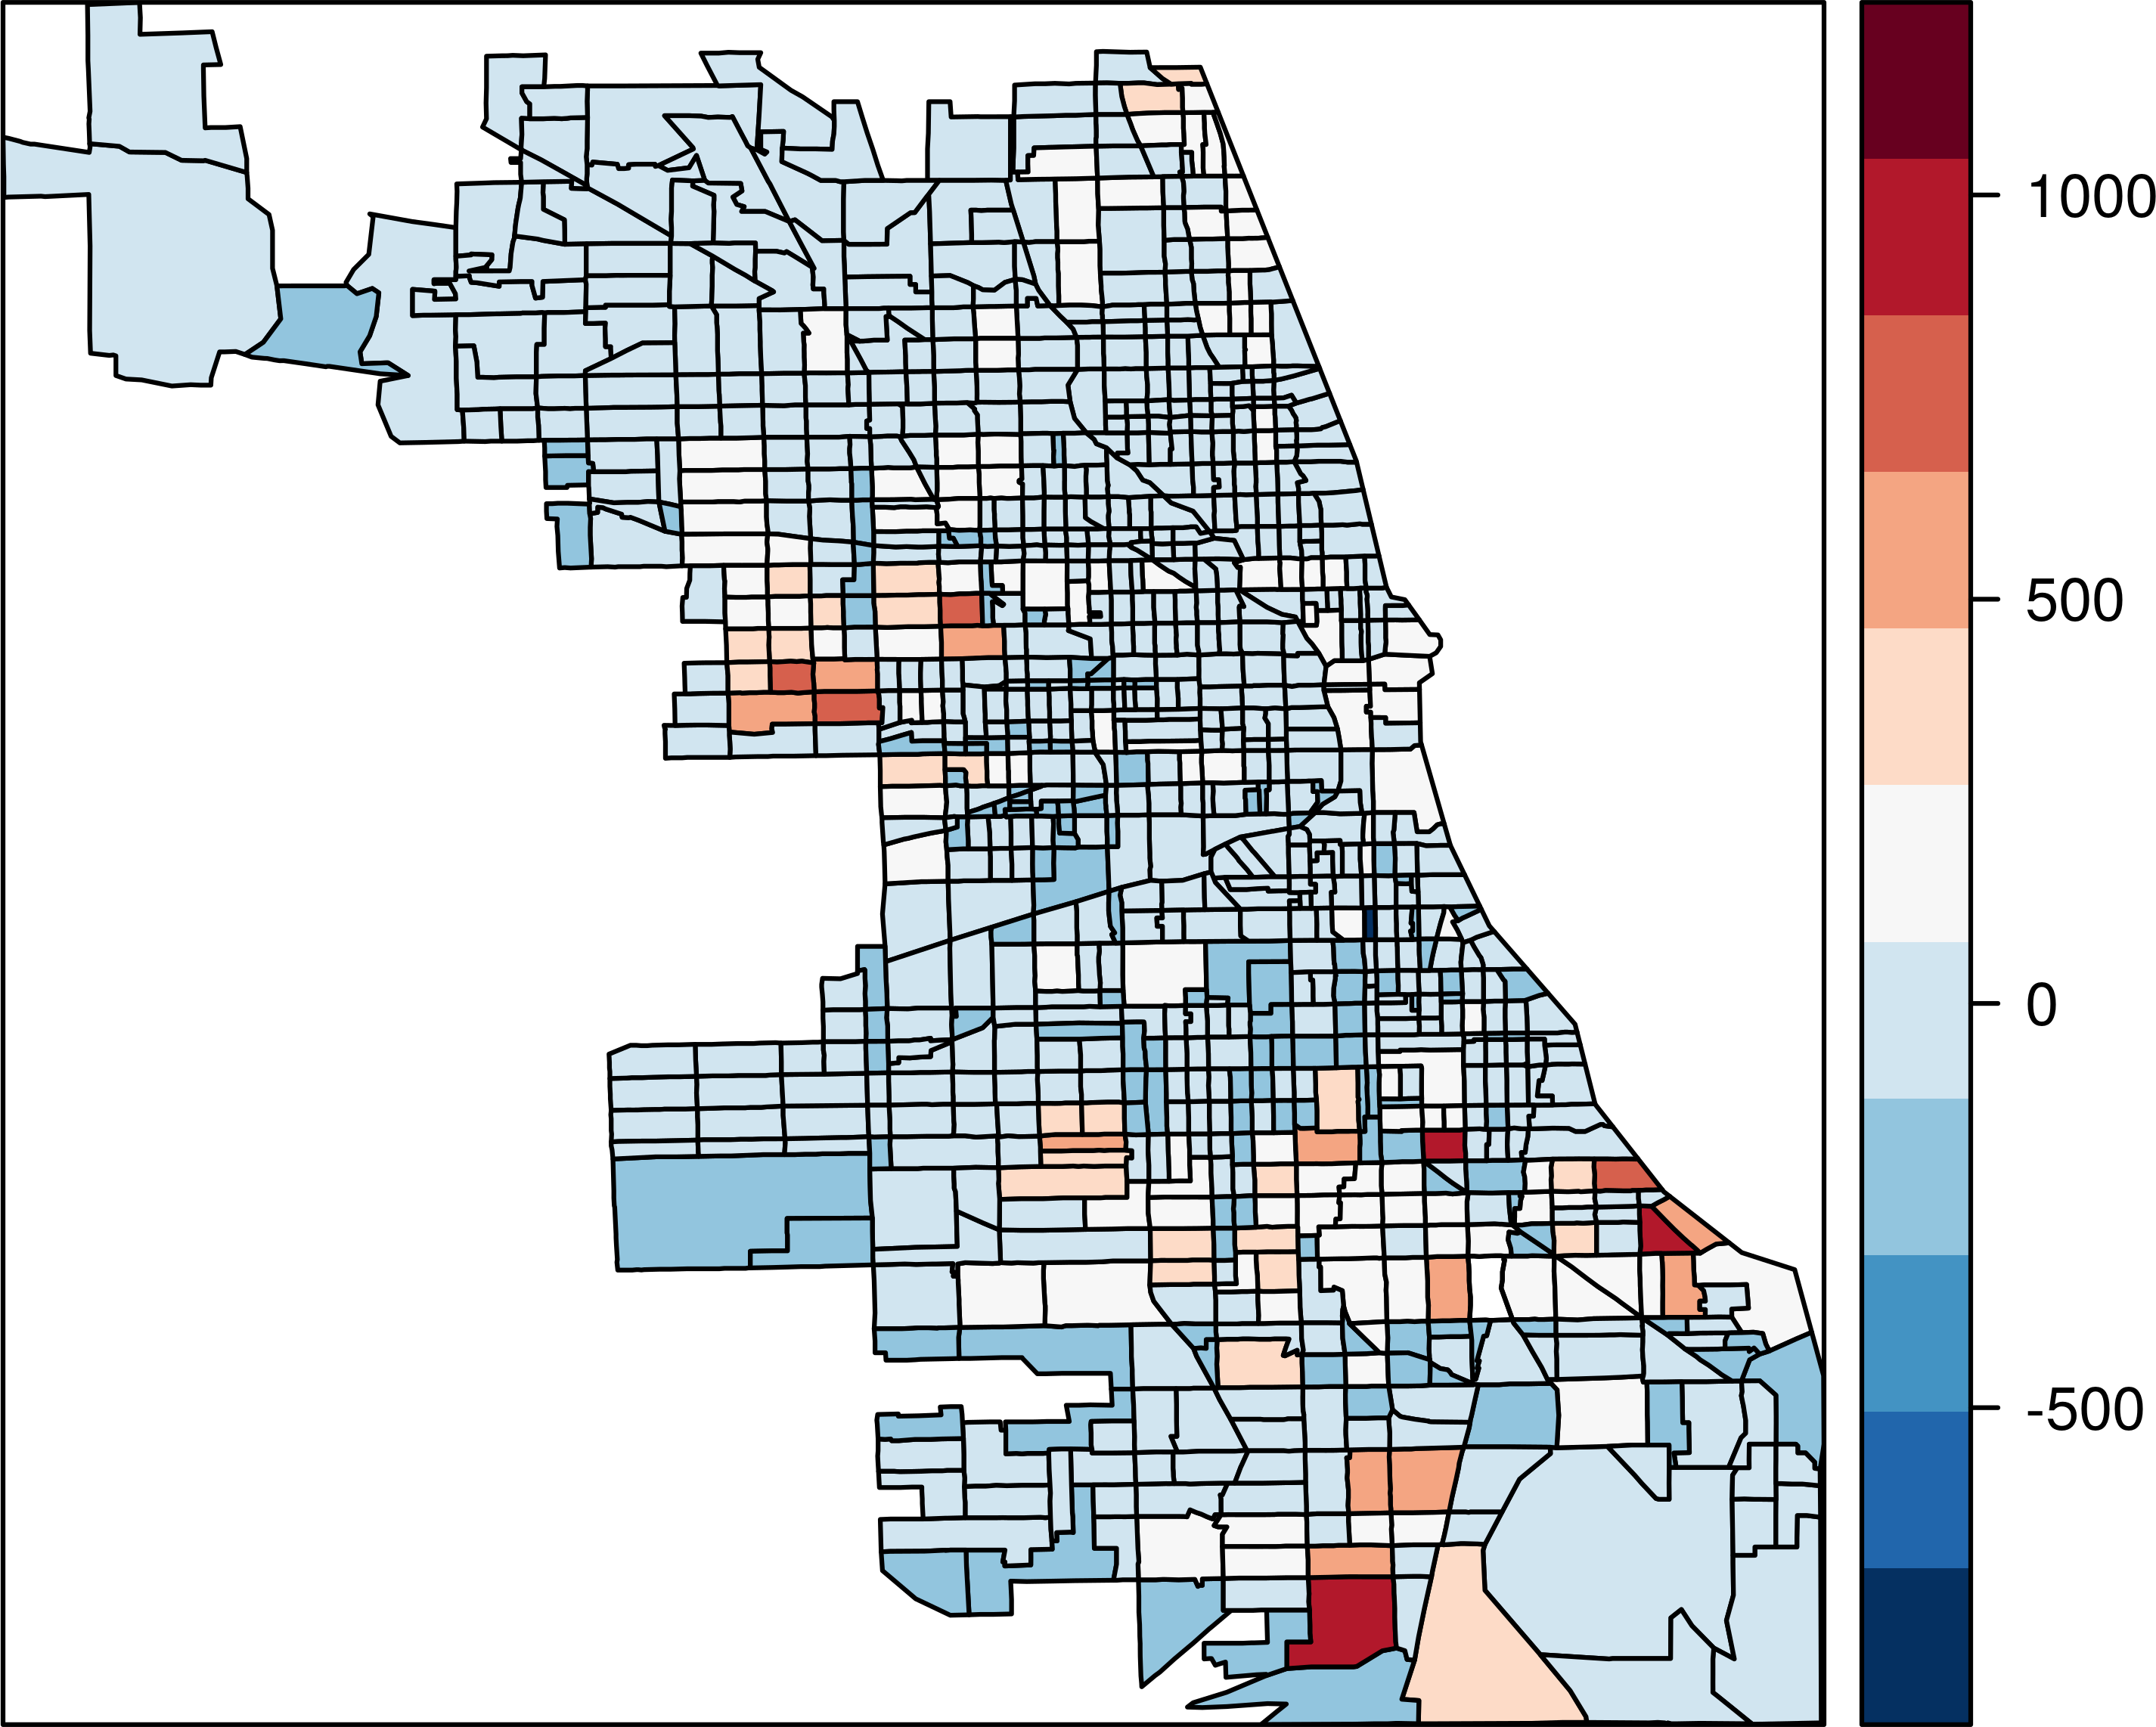
\includegraphics[width=0.49\linewidth]{sfiles/residual_plot-1} }\subfloat[Espacial\label{fig:residual_plot2}]{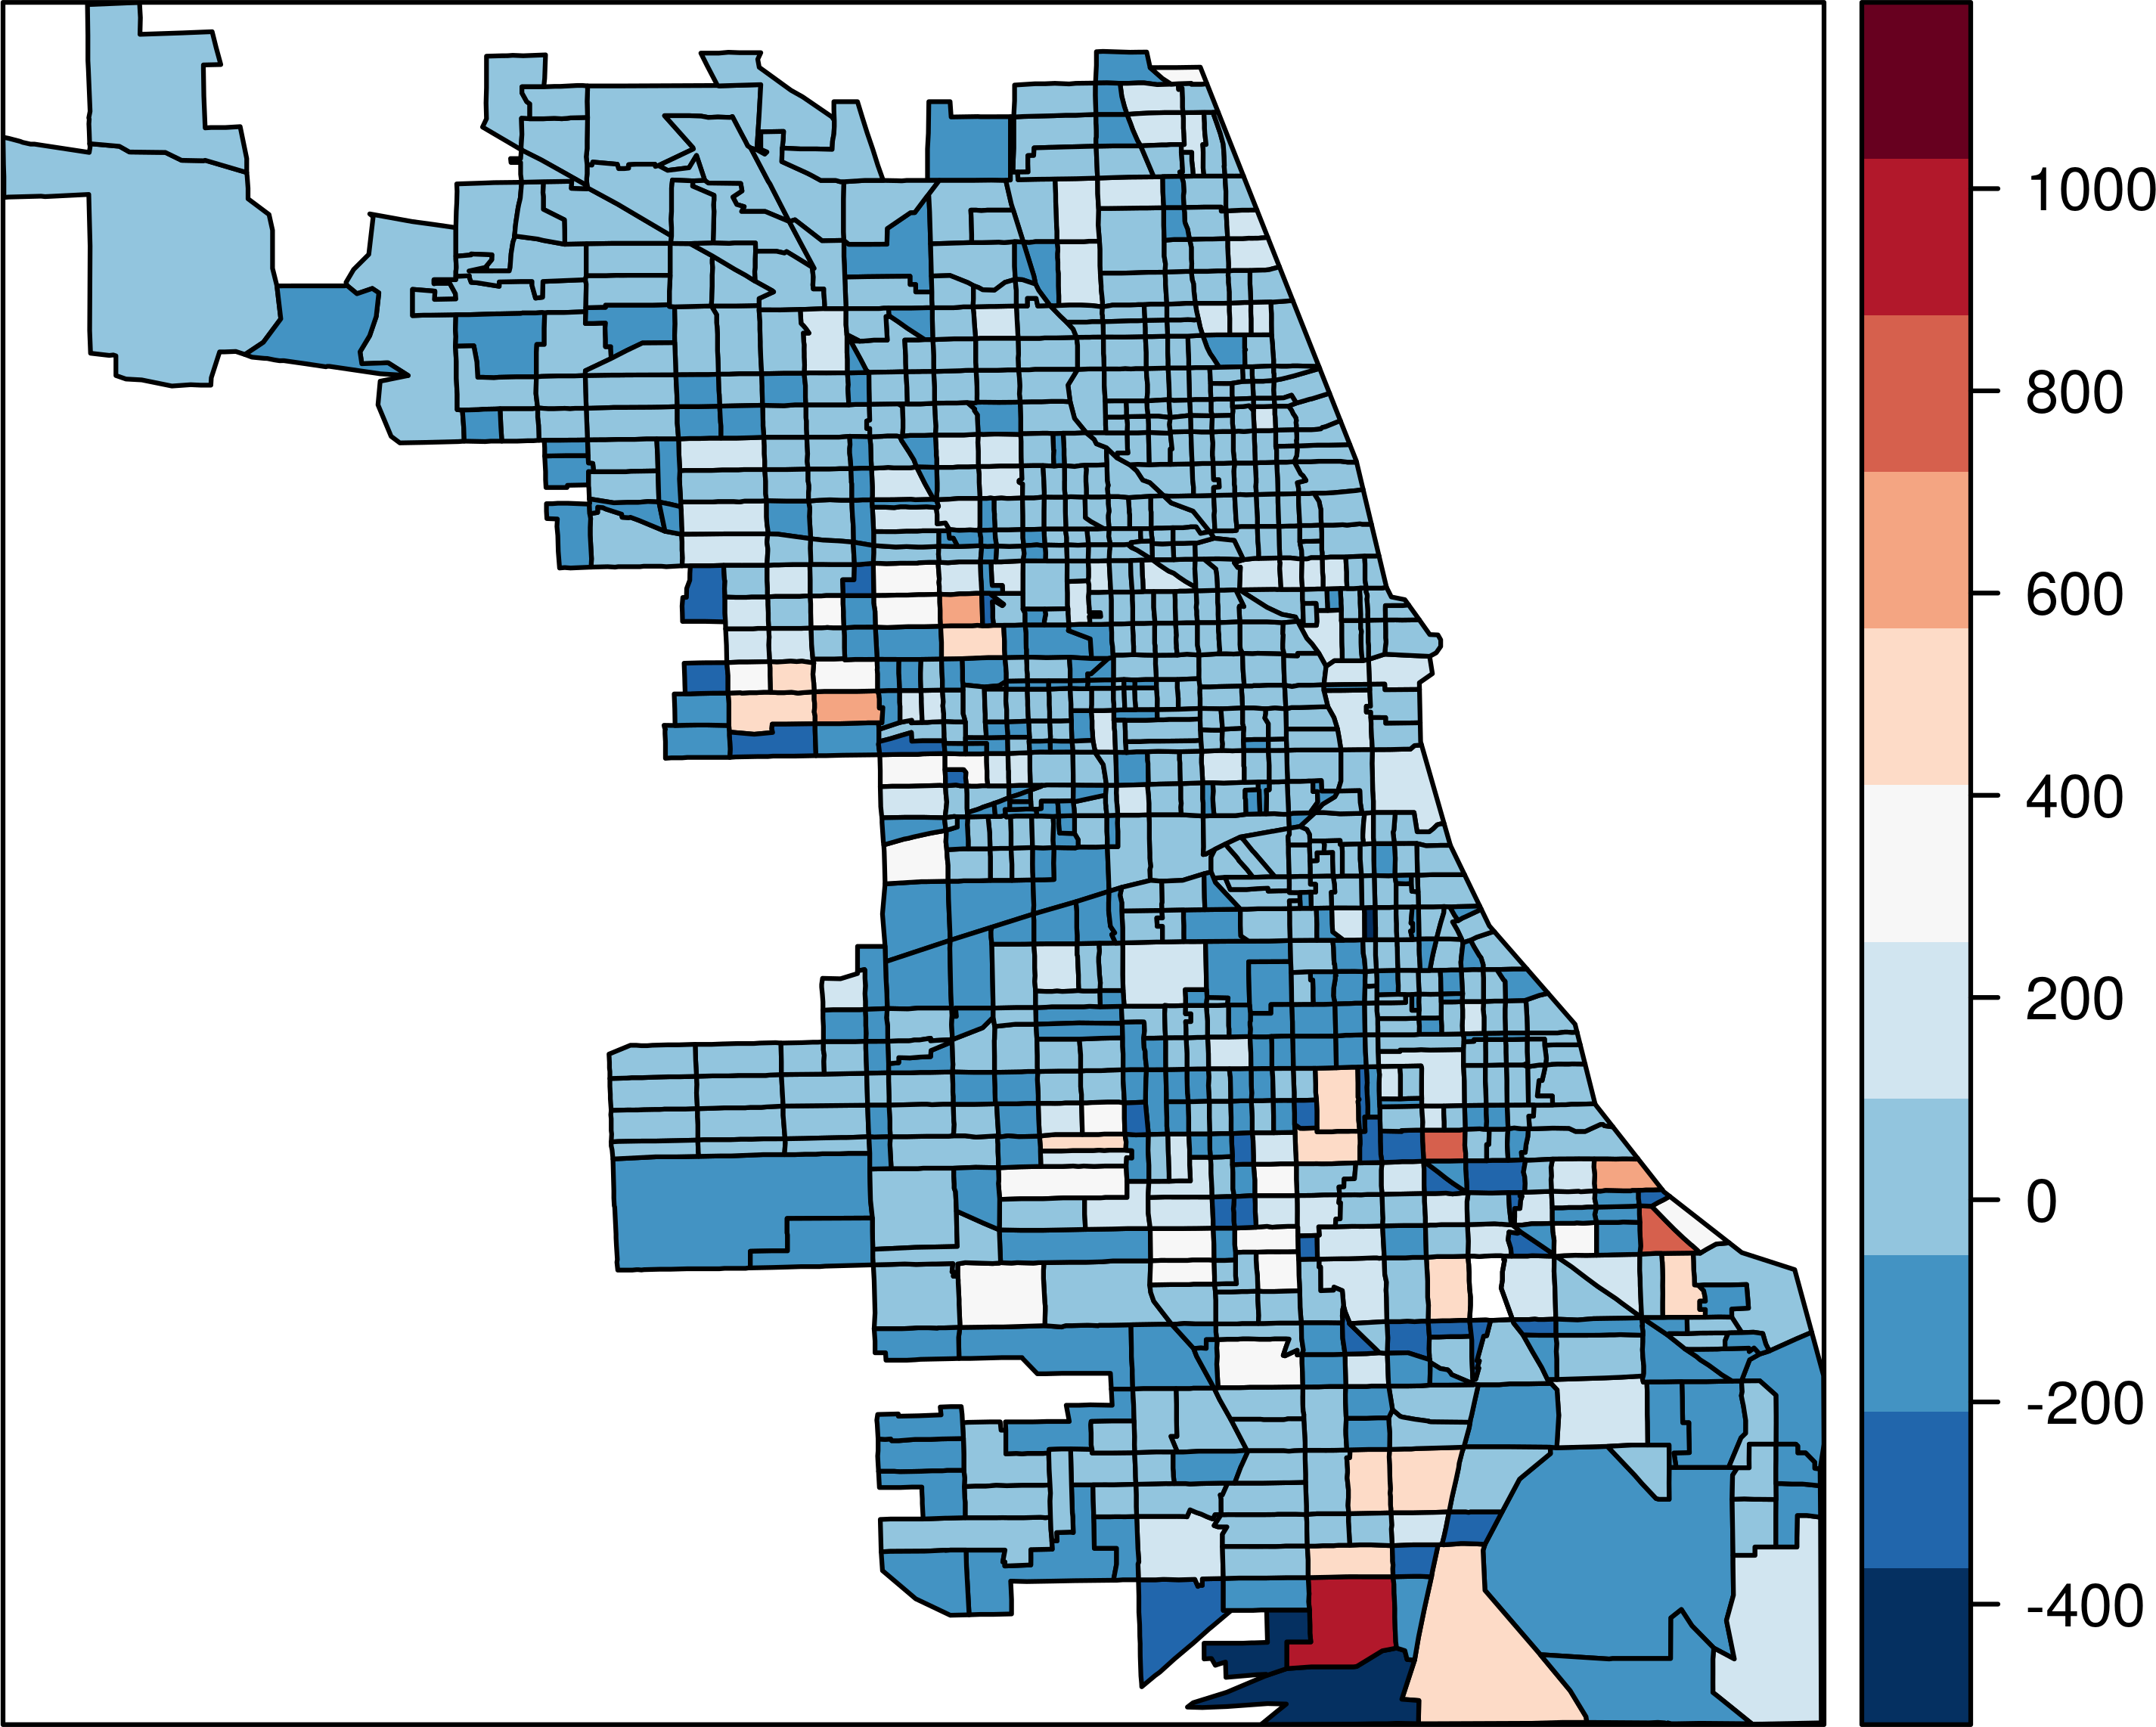
\includegraphics[width=0.49\linewidth]{sfiles/residual_plot-2} }

}

\caption{Resíduos das regressões linear e espacial}\label{fig:residual_plot}
\end{figure}

Os gráficos acima mostram que a autocorrelação espacial dos resíduos é
menor no modelo da variável dependente. Segundo SARMIENTO-BARBIERI
(\protect\hyperlink{ref-sarmiento-barbieri}{2016}), ``os gráficos de
resíduos ainda apresentam a presença de alguma autocorrelação espacial.
É muito provável que um modelo mais completo seja necessário. A
literatura se expandiu para modelos mais complexos''.

\subsection{Exemplo 2}\label{exemplo-2}

Neste exemplo serão utilizados dados da cidade de Boston (EUA),
elaborados por Harrison e Rubinfeld (1978). Nos dados são encontradas
variáveis de valores médios de imóveis, além de outras, como taxa de
crimes per capita em cada distrito.

\begin{Shaded}
\begin{Highlighting}[]
\KeywordTok{data}\NormalTok{(boston)}
\end{Highlighting}
\end{Shaded}

Inicialmente, monta-se um modelo de regressão linear ordinária, para
verificar a autocorrelação espacial dos resíduos.

\begin{Shaded}
\begin{Highlighting}[]
\NormalTok{boston_lm <-}\StringTok{ }\KeywordTok{lm}\NormalTok{(}\KeywordTok{log}\NormalTok{(CMEDV) }\OperatorTok{~}\StringTok{ }\NormalTok{RM }\OperatorTok{+}\StringTok{ }\NormalTok{LSTAT }\OperatorTok{+}\StringTok{ }\NormalTok{CRIM }\OperatorTok{+}\StringTok{ }\NormalTok{ZN }\OperatorTok{+}\StringTok{ }\NormalTok{CHAS }\OperatorTok{+}\StringTok{ }\NormalTok{DIS, }
                \DataTypeTok{data =}\NormalTok{ boston.c)}
\KeywordTok{summary}\NormalTok{(boston_lm)}
\end{Highlighting}
\end{Shaded}

\begin{verbatim}
## 
## Call:
## lm(formula = log(CMEDV) ~ RM + LSTAT + CRIM + ZN + CHAS + DIS, 
##     data = boston.c)
## 
## Residuals:
##      Min       1Q   Median       3Q      Max 
## -0.71552 -0.11248 -0.02159  0.10678  0.93024 
## 
## Coefficients:
##               Estimate Std. Error t value Pr(>|t|)    
## (Intercept)  2.8718878  0.1316376  21.817  < 2e-16 ***
## RM           0.1153095  0.0172813   6.672 6.70e-11 ***
## LSTAT       -0.0345160  0.0019665 -17.552  < 2e-16 ***
## CRIM        -0.0115726  0.0012476  -9.276  < 2e-16 ***
## ZN           0.0019330  0.0005512   3.507 0.000494 ***
## CHAS1        0.1342672  0.0370521   3.624 0.000320 ***
## DIS         -0.0302262  0.0066230  -4.564 6.33e-06 ***
## ---
## Signif. codes:  0 '***' 0.001 '**' 0.01 '*' 0.05 '.' 0.1 ' ' 1
## 
## Residual standard error: 0.2081 on 499 degrees of freedom
## Multiple R-squared:  0.7433, Adjusted R-squared:  0.7402 
## F-statistic: 240.8 on 6 and 499 DF,  p-value: < 2.2e-16
\end{verbatim}

Deve-se elaborar o vetor de pesos espaciais para a aplicação do teste de
Moran, como pode-se ver abaixo:

\begin{Shaded}
\begin{Highlighting}[]
\NormalTok{coords <-}\StringTok{ }\NormalTok{boston.utm}
\NormalTok{IDs <-}\StringTok{ }\KeywordTok{row.names}\NormalTok{(}\KeywordTok{as}\NormalTok{(boston.c, }\StringTok{"data.frame"}\NormalTok{))}
\NormalTok{boston_kdl <-}\StringTok{ }\KeywordTok{dnearneigh}\NormalTok{(coords, }\DataTypeTok{d1 =} \DecValTok{0}\NormalTok{, }\DataTypeTok{d2 =} \FloatTok{3.973}\NormalTok{, }\DataTypeTok{row.names =}\NormalTok{ IDs)}
\NormalTok{boston_W <-}\StringTok{ }\KeywordTok{nb2listw}\NormalTok{(boston_kdl)}
\KeywordTok{lm.morantest}\NormalTok{(boston_lm, boston_W)}
\end{Highlighting}
\end{Shaded}

\begin{verbatim}
## 
##  Global Moran I for regression residuals
## 
## data:  
## model: lm(formula = log(CMEDV) ~ RM + LSTAT + CRIM + ZN + CHAS +
## DIS, data = boston.c)
## weights: boston_W
## 
## Moran I statistic standard deviate = 5.8542, p-value = 2.396e-09
## alternative hypothesis: greater
## sample estimates:
## Observed Moran I      Expectation         Variance 
##     0.0700808323    -0.0054856590     0.0001666168
\end{verbatim}

O teste de Moran indica a autocorrelação espacial dos resíduos.

Alternativamente, a autocorrelação espacial pode ser pesquisada pelo
Teste do multiplicador de Lagrange:

\begin{Shaded}
\begin{Highlighting}[]
\KeywordTok{lm.LMtests}\NormalTok{(boston_lm, boston_W, }\DataTypeTok{test =} \StringTok{"all"}\NormalTok{)}
\end{Highlighting}
\end{Shaded}

\begin{verbatim}
## 
##  Lagrange multiplier diagnostics for spatial dependence
## 
## data:  
## model: lm(formula = log(CMEDV) ~ RM + LSTAT + CRIM + ZN + CHAS +
## DIS, data = boston.c)
## weights: boston_W
## 
## LMerr = 26.124, df = 1, p-value = 3.201e-07
## 
## 
##  Lagrange multiplier diagnostics for spatial dependence
## 
## data:  
## model: lm(formula = log(CMEDV) ~ RM + LSTAT + CRIM + ZN + CHAS +
## DIS, data = boston.c)
## weights: boston_W
## 
## LMlag = 46.723, df = 1, p-value = 8.175e-12
## 
## 
##  Lagrange multiplier diagnostics for spatial dependence
## 
## data:  
## model: lm(formula = log(CMEDV) ~ RM + LSTAT + CRIM + ZN + CHAS +
## DIS, data = boston.c)
## weights: boston_W
## 
## RLMerr = 5.0497, df = 1, p-value = 0.02463
## 
## 
##  Lagrange multiplier diagnostics for spatial dependence
## 
## data:  
## model: lm(formula = log(CMEDV) ~ RM + LSTAT + CRIM + ZN + CHAS +
## DIS, data = boston.c)
## weights: boston_W
## 
## RLMlag = 25.649, df = 1, p-value = 4.096e-07
## 
## 
##  Lagrange multiplier diagnostics for spatial dependence
## 
## data:  
## model: lm(formula = log(CMEDV) ~ RM + LSTAT + CRIM + ZN + CHAS +
## DIS, data = boston.c)
## weights: boston_W
## 
## SARMA = 51.773, df = 2, p-value = 5.723e-12
\end{verbatim}

Finalmente, elabora-se o modelo da variável dependente com o vetor de
pesos espaciais.

\begin{Shaded}
\begin{Highlighting}[]
\NormalTok{boston_lag <-}\StringTok{ }\KeywordTok{lagsarlm}\NormalTok{(}\KeywordTok{log}\NormalTok{(CMEDV) }\OperatorTok{~}\StringTok{ }\NormalTok{RM }\OperatorTok{+}\StringTok{ }\NormalTok{LSTAT }\OperatorTok{+}\StringTok{ }\NormalTok{CRIM }\OperatorTok{+}\StringTok{ }\NormalTok{ZN }\OperatorTok{+}\StringTok{ }\NormalTok{CHAS }\OperatorTok{+}\StringTok{ }\NormalTok{DIS, }
                       \DataTypeTok{data =}\NormalTok{ boston.c, }\DataTypeTok{listw =}\NormalTok{ boston_W)}
\KeywordTok{summary}\NormalTok{(boston_lag)}
\end{Highlighting}
\end{Shaded}

\begin{verbatim}
## 
## Call:lagsarlm(formula = log(CMEDV) ~ RM + LSTAT + CRIM + ZN + CHAS + 
##     DIS, data = boston.c, listw = boston_W)
## 
## Residuals:
##       Min        1Q    Median        3Q       Max 
## -0.661775 -0.110275 -0.022402  0.093404  0.889062 
## 
## Type: lag 
## Coefficients: (asymptotic standard errors) 
##                Estimate  Std. Error  z value  Pr(>|z|)
## (Intercept)  1.94228257  0.19267675  10.0805 < 2.2e-16
## RM           0.10158291  0.01655116   6.1375 8.382e-10
## LSTAT       -0.03227679  0.00192717 -16.7483 < 2.2e-16
## CRIM        -0.01033127  0.00120283  -8.5891 < 2.2e-16
## ZN           0.00166558  0.00052968   3.1445  0.001664
## CHAS1        0.07238573  0.03608725   2.0059  0.044872
## DIS         -0.04285133  0.00655158  -6.5406 6.127e-11
## 
## Rho: 0.34416, LR test value: 37.426, p-value: 9.4936e-10
## Asymptotic standard error: 0.051967
##     z-value: 6.6226, p-value: 3.5291e-11
## Wald statistic: 43.859, p-value: 3.5291e-11
## 
## Log likelihood: 98.51632 for lag model
## ML residual variance (sigma squared): 0.03944, (sigma: 0.1986)
## Number of observations: 506 
## Number of parameters estimated: 9 
## AIC: -179.03, (AIC for lm: -143.61)
## LM test for residual autocorrelation
## test value: 1.9852, p-value: 0.15884
\end{verbatim}

Verifica-se no sumário acima que a autocorrelação espacial foi eliminada
do modelo, dado que o p-valor resultou maior que 5\% (0,15884).

\section{CONCLUSÃO}\label{conclusao}

O sistema \textbf{R} mostrou-se adequado para a elaboração de modelos de
regressão espacial, com funções específicas para isso, que podem ser
utilizadas com facilidade, apenas fornecendo-se uma fórmula comum de
regressão linear, os dados, e uma matriz de pesos espaciais.

O \textbf{R} também é eficiente para a construção da própria matriz de
pesos espaciais, com várias funções para isto. A utilização de modelos
de regressão espacial deverá ser cada vez maior na área de avaliação de
imóveis no futuro e o sistema \textbf{R} pode vir a se tornar uma das
ferramentas mais utilizadas, pela sua grande facilidade de uso, pela
grande quantidade de pacotes relacionados à área e até pelo fato de ser
um software livre.

\section*{REFERÊNCIAS}\label{referencias}
\addcontentsline{toc}{section}{REFERÊNCIAS}

\hypertarget{refs}{}
\hypertarget{ref-sarmiento-barbieri}{}
SARMIENTO-BARBIERI, Ignacio. 2016. \emph{An Introduction to Spatial
Econometrics in R}. Illinois: University of Illinois.
\url{http://www.econ.uiuc.edu/~lab/workshop/Spatial_in_R.html}.

\hypertarget{ref-trivelloni07}{}
TRIVELLONI, Carlos Alberto Peruzzo. 2007. ``COMPARAÇÃO de Modelos
Inferenciais Tradicionais E Espaciais Utilizando Diferentes Variáveis de
Localização.'' \emph{XIV COBREAP}. \url{https://goo.gl/tpk5kW}.


\end{document}
